\chapter{Założenia projektowe}
W rozdziale opisano główny problem oraz potencjalne ścieżki prowadzące do jego rozwiązania. Zamieszczono w nim również wynik przeprowadzonej analizy wymagań funkcjonalnych i niefunkcjonalnych dla mającej powstać aplikacji. Zaproponowano ponadto makiety interfejsu użytkownika oraz przedstawiono narzędzia i technologie wybrane do realizacji celu pracy.

\section{Zarys architektury systemu}
% Описание проблемы:
% Существует проблема найти рабочую станцию зарядки, когда остается мало зарядки в автомобиле.
% Станция может не работать, плохо заряжать, может быть установлена так, что ей невозможно пользоваться, 
% различные сервисы, зачастую, ориентируются на конкретную фигрму заправок и могут не иметь самую актуальную информацию о появлении станций других производителей.
% Хочется просто взять телефон и прямо на карте увидеть где есть станции и посмотреть о ней отзывы реальных людей.

% В результате работы должно быть создано мобильное приложение в которм:
% Водители жлекторомобилей могут легко и быстро находить ближайшие зарядные станции и выбирать лучшую.
% Владельцы стнаций могут добавлять свои станции, что даст им дополнительную рекламу.
% Для определения качества станции должна использоваться система актуальных коментариев и оценок зарегестрированных пользователей.
% Каждый пользователь должен иметь собственный аккаунт для возможности пользоваться приложениемю
% Эта система позволит повысить качество зарядных пунктов.
% Это приложение полнстью поддеживается сообществом: создание и оценка станций производится пользователями.

% В пользовательском интерфейсе, которым я вляется мобильное приложение, должна быть интегрирована карта для упрощения поиска и создания мест.
% Должна быть реализована система регистарции и входа.
% Кроме пользовательского интерфейса долен быть реализована серверная часть, для обработки действий пользователей.
% А также база данных дляхранения станций и коментариев.

% Предположительный макет сервиса:
\paragraph{Opis problemu:}
Istnieje problem ze znalezieniem dobrej stacji ładującej pojazdy elektryczne.
Stacja może nie działać, źle ładować, może być zainstalowana tak, że nie można jej używać.
Większość istniejących aplikacji najczęściej ma dostęp tylko do stacji konkretnych firm i mogą nie mieć najbardziej aktualnych informacji o pojawieniu się stacji innych producentów oraz ocen rzeczywistych użytkowników.
Istnieje chęć po prostu wziąć telefon i zobaczyć bezpośrednio na mapie, gdzie są stacje i zobaczyć recenzje prawdziwych ludzi na ten temat.

\paragraph{W wyniku pracy ma powstać aplikacja mobilna w której:}
Kierowcy samochodów elektrycznych mogą łatwo i szybko znaleźć najbliższe stacje ładowania i wybrać najlepszą.
Właściciele stacji mogą dodawać swoje stacje, co da im dodatkową reklamę.
Aby określić jakość stacji, należy użyć systemu aktualnych komentarzy i ocen zarejestrowanych użytkowników.
Każdy użytkownik musi posiadać własne konto, aby móc korzystać z aplikacji.
Taki system może spowodować zwiększenie jakośi punktów ładowania pojazdów elektrycznych.
Ta aplikacja musi być w pełni wspierana przez społeczność: tworzenie i ocena stacji odbywa się przez użytkowników.

\paragraph{Przypuszczalny układ serwisu:}
Interfejs użytkownika, którym jest aplikacja mobilna, musi mieć zintegrowaną mapę, aby ułatwić wyszukiwanie i tworzenie miejsc.
Należy wdrożyć system rejestracji i logowania.
Oprócz interfejsu użytkownika musi być zaimplementowana część serwerowa do obsługi działań użytkowników.
A także baza danych do przechowywania stacji i komentarzy. Ten układ widać na rysunku \ref{fig:zarysuskladuserwisu}.
\begin{figure}[ht]
    \centering
        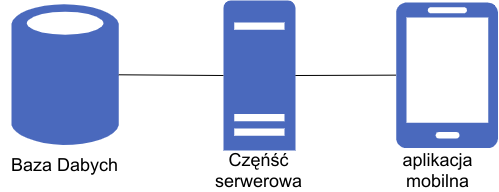
\includegraphics[width=0.4\linewidth]{rys02/uklad_wstepny.png}
        \caption{zarys uskladu serwisu \cite{diagrams_net}}
    \label{fig:zarysuskladuserwisu}
\end{figure}\newline

\section{Analiza wymagań}
\subsection{Wymagania funkcjonalne}
W tabeli \ref{tab:wymaganiafunkcjonalne} przedstawione wymagania funkc do aplikacji mobilnej razem z celem ich wdrożenia.
\begin{table}[htb] \small
    \caption{Wymagania funkcjonalne}
    \label{tab:wymaganiafunkcjonalne}
    \begin{tabular}{| m{0.5cm} | m{7cm} | m{7cm} |} 
    \hline
    № & Opis & Cel \\
    \hline
    1 & Użytkownik loguje się do własnego konta. & Umożliwia korzystanie z funkjalności aplikacji. \\ 
    \hline
    2 & Użytkownik rejestruje się. & Założenie konta tworzy nowy wpis w bazie danych pozwalający na logowanie. \\ 
    \hline
    3 & Użytkownik wyszkuję stacje ładownicze obok wybranego miejca  & dać użytkownikowi możliwość wyboru dogodnej dla niego stacji \\
    \hline
    4 & Użytkownik ma możliwość określenia własnej pozycji & Wyszukiwanie wygodniejszych stacji bardziej intuicyjne dla użytkownika  \\
    \hline
    5 & Użytkownik ma możliwość przęgliądania mapy razem ze swoją lokalizacją oraz stacji łaowniczych obok wybranego mijsca. & Ułatwienie wyszukiwania najwygodniejszej stacji ładowniczej. \\
    \hline
    6 & Użytkownik ma możliwość wyszukiwania stacji ładowniczej według słów kluczowych & Wyszukiwanie najwygoniejszej stacji z punktu widzenia typu lub nazwy stacji \\
    \hline
    7 & Użytkownik ma możliwość przeglądania informacji dotyczącej stacji ładowniczej, w tym liku oceny i komentarzy innych użytkowników & Podjęcie decyzji i dobór odpowiedniej dla użytkownika stacji ładowniczej \\
    \hline
    8 & Użytkownik ma możliwość wystawienia oceny i napisania komentarzy do wybranej stacji ładowniczej & Określenie jakości stacji. Pozwala na aktualizację danuch dotyczących stacji ladowniczej \\
    \hline
    9 & Użytkownik ma możliwość dowdawania (oznaczenia, tworzenie) nowej stacji ładowniczej & Aktualizacja informacji o dostępnych stacjach \\
    \hline
    10 & Użytkownik, który stworzył stację, ma możliwość zmiany informacji o tej stacji ładowniczej & Aktualizacja informacji istniejącej statji \\
    \hline
\end{tabular}
\end{table}

\paragraph{Diagram Przypadków użycia\newline}
Diagram przypadków użycia (rys.~\ref{fig:usecasediagram}) graficznie pokazuje użytkowników oraz funkcje aplikacji dostępne do różnych rodzajów użytkowników (w tym przypadku jeden rodzaj).
\begin{figure}[ht]
    \centering
        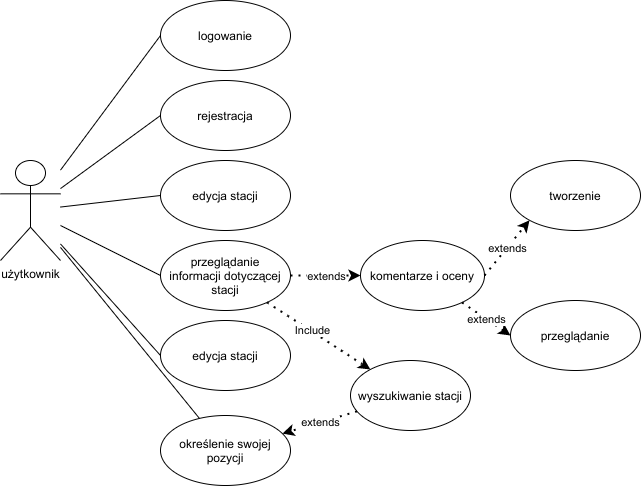
\includegraphics[width=0.7\linewidth]{rys02/use_case_diagram.png}
        \caption{dagram przypadków uzycia \cite{diagrams_net}}
    \label{fig:usecasediagram}
\end{figure}

\subsection{Wymagania niefunkcjonalne}
W tabeli \ref{tab:wymaganianiefunkcjonalne} przdstawione wymagania niefunkcjonalne: krótki opis wymagania, typ (jakiej dziedziny to dotyczy) oraz uwagi do tego wymagania.
\begin{table}[htb] \small
    \caption{Wymagania niefunkcjonalne}
    \label{tab:wymaganianiefunkcjonalne}
    \begin{tabular}{| m{0.5cm} | m{3cm} | m{5.75cm} | m{5.75cm} |} 
    \hline
    № & typ & Opis & Uwagi \\
    \hline
    1 & Bezpiczeństwo & Hasła muszą być przechowywane w biezpicznej formie & Hasła nie przchowyją się w pierwotnej formie, tylko w formie zaszyfrowanej \\ 
    \hline
    2 & Bezpiczeństwo & Małe ryzyka przechwytywania hasła przez trzecich osób podczas komunikacji interfejsu użytkownika i części serwerowej & Autentykacja użytkownika na serwerze powinna zachodzić za pomocą tokenów \\ 
    \hline
    3 & Przenoszlność & wdrożenie systemu powinno być szybkie i łatwe & \\ 
    \hline
    4 & Konfigurowalność & Zmiana ustaleń bez konieczosści rekompilacji części serwerowej & Zarządzaniem portu na którym działa część serwerowa, wymiana adresu oraz nazwy kolekcji bazy danuch, musi być możliwa za pomocą pliku konfiguracyjnego \\ 
    \hline
    5 & Estetyczne & Przyjazny interfajs użytkownika & Intuicyjny i zrozumiały interfejs \\ 
    \hline
    6 & Ergonomia & Interfejs w języku angielskim & Możliwość kożystania z aplikacji przez dużą libzi \\
    \hline
    7 & Przenoszlność & Aplikacja mobilna musi działać na 90\% lub więcej telefonów pracujących na systemie Android & Możliwość kożystania z aplikacji przez dużą ilość ludzi \\
    \hline
    8 & Estetyczne & kolory muszą być odpowiednio dopasowane & Wykorzystanie małej dopasowanych do sobie ilośći kolorów  \\
    \hline
    9 & Wydajność & Srzybka reakcja systemu & System musi szybko reagować na działania użytkownika \\
    \hline
    10 & Informatywność & System powinien powiadomiać o błędach i sukcesach  & Podczas rażądzania systemem użytkownik powinin zawze wiedzieć jaki wynik jego działania \\
    \hline
    11 & Ergonomia & Wykorzystanie z aplikacji mobilnej za pomocą jednej ręki & Przyciski muszą znajdować się w dolnej części ekranu lub znajdować się w dostępnym miejscu \\
    \hline
    12 & Estetyczne & Wszystkie elementy muszą być w jednym stylu & Niedopuszczalne jest użycie różnych czcionek oraz ciągłej zmiany kolorów \\
    \hline
    13 & Dostęp & Część serwerowa zrobiona zgodnie z regułami Rest (ang. \textit{Representational State Transfer}) API (ang. \textit{Application Programming Interface}) & Przestrzeganie się Best Prakties Rest API \cite{rest_api_best}] \\
    \hline
    14 & Ergonomia & Dla realizacji mapy wykorzystuję się Google Maps[index] & Ułatwia rozumienie interfejsu dla użytkowników \\
    \hline
\end{tabular}
\end{table}
\newpage
\subsection{Nażędzia i technologie}
Do sworzenia aplikacji mobilnej, części serwerowej oraz bazy daych zostały wybrane następujące narzędzia i technologie:
\begin{multicols}{3}
\begin{itemize}
    \item Visual Studio Code;
    \item Go;
    \item REST API;
    \item JWT;
    \item MongoDB;
    \item Redis;
    \item Android Studio;
    \item Gradle;
    \item Android SDK;
    \item Java JDK 8;
    \item RxJava 2;
    \item Google Cloud Platform;
    \item GMS;
    \item Docker;
\end{itemize}
\end{multicols}
\paragraph{Visual Studio Code} \cite{vscode} to darmowy edytor kodu źródłowego, który został wyprodukowany przez Microsoft. Działa na systemach Windows, Linux, macOS. Jest rozszerzalny za pomocą plug-inów.
Lista podtrzymywanych języków i możliwości jest dość wielka i może być rozszerzona za pomocą plug-inów. Kilka funkcji: podświetlanie składni, IntelliSense, refaktoryzacja, debugowanie i inne.

\paragraph{Go} (golang) \cite{golang1,golang2,golang3,godoc} jest językiem programowania. Kompilowany, wielowątkowy. Stworzony przez Google. Kod tego języku może być kompilowany do Linux, Windows, macOS, FreeBSD, Android i inne.
Język jest przeznaczony do budowania serwisów z wysokim obciążeniem i efektywnością, które pracują na systemach rozproszonych z wielowątkowymi procesorami.

\paragraph{REST API} (ang. \textit{REpresentational State Transfer}) (ang. \textit{Application Programming Interface}) \cite{rest_api,rest_api_best} Jest to popularne podejście w architekturze tworzenia interfejsów programistycznych.
Podstawowe zasady to: architektura klient-serwer (na przykład przydzielamy klienta i magazyn danych), brak stanu (serwer nie przechowuje stanu klienta, wszystkie potrzebne informacje są wysyłane wraz z żądaniem),
buforowalność (buforowanie danych jest dozwolone, jeśli w odpowiedzi jest na to zgoda), jednorodność interfejsu (ograniczenia stylu pisania), wielopoziomowość systemu (komponenty systemu mają bezpośredni dostęp tylko do sąsiednich warstw), łatwość rozszerzenia funkcjonalności (opcjonalnie).

\paragraph{JWT} (ang. \textit{JSON Web Token}) \cite{jwt} jest standardem, który jest przeznaczony do tworzenia tokenów dostępu. Za pomocą JWT sprawdza się, czy wchodzące dane zostały wysłane przez autoryzowane źródło.
Składa się z trzech części: nagłówek (informacja o tym, w jaki sposób odszyfrować token), dane (zaszyfrowane dane) oraz sygnatura. Każdy taki token ma czas działania. Nie może być oznaczony jako nieroboczy, dopóki nie skończy się czas jego działania.

\paragraph{MongoDB} \cite{mongoDB,mongoDB_doc,mongodb_habr} jest NoSQL (ang. \textit{Not only Structured Query Language}) rozwiązaniem do przechowywania danych. Dane przehowywane w formacie BSON (ang. \textit{Binary JavaScript Object Notation}).
Format licencji SSPL (ang. \textit{Server Side Public License}). Wykorzystuje technikę segmentacji obiektów bazy danych, co pozwala na bilansowanie obciążenia.

\paragraph{Redis} \cite{redis} system zarządzania bazami danych klasy NoSQL, który współpracuje ze strukturami danych typu ,,klucz-wartość''. Najczęściej używa sie do implementacji baz dabych, pamięci podręcznej, brokerów wiadowmości.

\paragraph{Android Studio} \cite{android_doc,android_studio} zintegrowane środowisko programistyczne, które zostało wyprodukowane przez JetBrains na podstawie IelliJ IDEA, do budowania aplikacji na platformie Android. Jest dostępna do systemów Windows, Linux, macOS. Jest udostępniona za pomocą bezpłatnej licencji Apache 2.0.

\paragraph{Gradle} \cite{gradle,gradle_android_doc} jest systemem automatycznego budowania aplikacji oraz zarządzania zależnościami, który służy do uproszczenia pracy z językiem Java.

\paragraph{Android SDK} \cite{android_studio} (ang. \textit{Software development kit}) jest narzędziem do tworzenia aplikacji mobilnych dla systemów na bazie Android, które został wyprodukowane przez Google.
Ten zestaw SKD zawiera nażędzia programistyczne: zestaw bibliotek Android i Java, emulator telefonu, debugger, dokunentację, szablony prostych aplikacji.

\paragraph{Java JDK 8} (and. \textit{Java Development Kit}) \cite{java_doc} jest zestawem programisty do programowania w języku Java. Zawiera: kompilator języka Java, przykłady, dokumentację, system uruchomiania koda Java (JDK (ang. \textit{Java Runtime Environment})).
Java jest językiem ogólnego zastosowania, obiektowym, krosplatformowym, dzięki uruchomianiu się kodu na maszynie wirtualnej. Został wyprodukowany przez Sun Microsystems.
Przy tworzeniu aplikacji został użyty język wersji 8, ponieważ kompatybilność tej wersji jest bardzo wysoka.

\paragraph{RxJava 2} jest to biblioteka pozwalająca na stosowanie reaktywnego programowania w języku Java. Programowanie reaktywne jest paradygmatem programowania pozwalającym na programowanie z asynchronicznymi strumieniami (sekwencja stałych zderzeń, które posortowane według czasu) danych.
Ta biblioteka jest bardzo przydatna na przykład, żeby interfejs użytkownika ciągle był dostępny do użycia, nawet w podczas obliczania jakiejś logiki, na przykład oczekiwanie odpowiedzi od serwera.

\paragraph{Google Cloud} \cite{google_cloud} jest pakietem Google usług w chmurze. Ten serwis pozwala na wykorzystanie serwisów Google Search, Gmail, przechowywanie plików, Youtube, obliczenie i przechowywanie danych, uczenie maszynowe i inne usługi, z których korzysta Google w swoich projektach.
Usługa ta jest płatna. Różne części mają różne koszty w zależności od ilości zapytań do serwisów Google. Jeśli koszty użycia tych serwisów mniej niż 200 dolarów miesięcznie, Google nie pobiera opłaty. W tej pracy inżynierskiej został wykorzystany serwis Static Maps \cite{google_cloud_pricing}.
Ten serwis jest darmowy przy tworzeniu oprogramowania do telefonów (Android Maps SDK for Android (ang. \textit{Maps Software development kit for Android}) \cite{maps_sdk}).

\paragraph{GMS}  (and. \textit{Google Mobile Services}) jest to zestaw aplikacji dostarczonych przez Google: Goole Maps, Google Paly Store, Gmail Google Drive Google Duo, Google Chrome, Google Photos, Google TV, YOutube, Youtube Music.

\paragraph{Docker} \cite{docker,docker_doc} jest to oprogramowanie przeznaczone do automatyzacji wdrażania i zarządzania aplikacjami. Aplikacje uruchamiają się w kontenerach. Docker pozwala na upakowanie aplikacji oraz wszystkich zależności w niezależny od podstawowego systemu kontener, który może być łatwo przeniesiony na dowolny *nix system.

% Jako Baza danych wykorzystuje się NoSQL (ang. (ang. \textit{Not only Structured Query Language}) baza danych MongoDB \cite{mongoDB,mongoDB_doc}.
% Część serwerowa napisana w języku Go \cite{golang1,golang2,golang3,godoc} w architekturze Rest API \cite{rest_api_best}.
% Część serwerowa i Baza Danych muszą uruchamiać się w Docker kontenerze \cite{docker,docker_doc}.
% Aplikacja mobilna działa w systemie Android za pomocą Android Studio \cite{android_doc,android_studio,gradle,gradle_android_doc} w języku Java \cite{java_doc}.
% Dla realizacji Google Maps w aplikacji mobilnej wykorzystuję się serwis Google Cloud \cite{google_cloud} Maps SDK for Android (ang. \textit{Maps Software development kit for Android}) \cite{maps_sdk}.
% 
\subsection{Makiety interfejsu użytkownika}
Po analizie wymagań zostały stworzone możliwe makiety aplikacji, która ma powstać.

Na dole ekranu aplikacji znajduje się główne menu zawierające 4 pozycje: mapę, wyszukiwanie stacji, tworzenie stacji i parametry.
Na rysunku \ref{fig:search_makiet}a przedstawiono pierwszy etap wyszukiwania stacji ładowania.
Pod polem wyszukiwania znajduje się rozwijane menu, które pozwala wybierać typ wyszukiwania, w tym wyszukiwanie na podstawie pozycji użytkownika oraz nazwy i opisu stacji.
Poniżej znajduje się możliwość do zmiany dystansu wyszukiwania oraz przycisk wyszukiwania.
\begin{figure}[ht]
	\centering
  \begin{tabular}{@{}rl@{\hspace{10mm}}rl@{}}
  a) & \vtop{\vskip-2ex\hbox{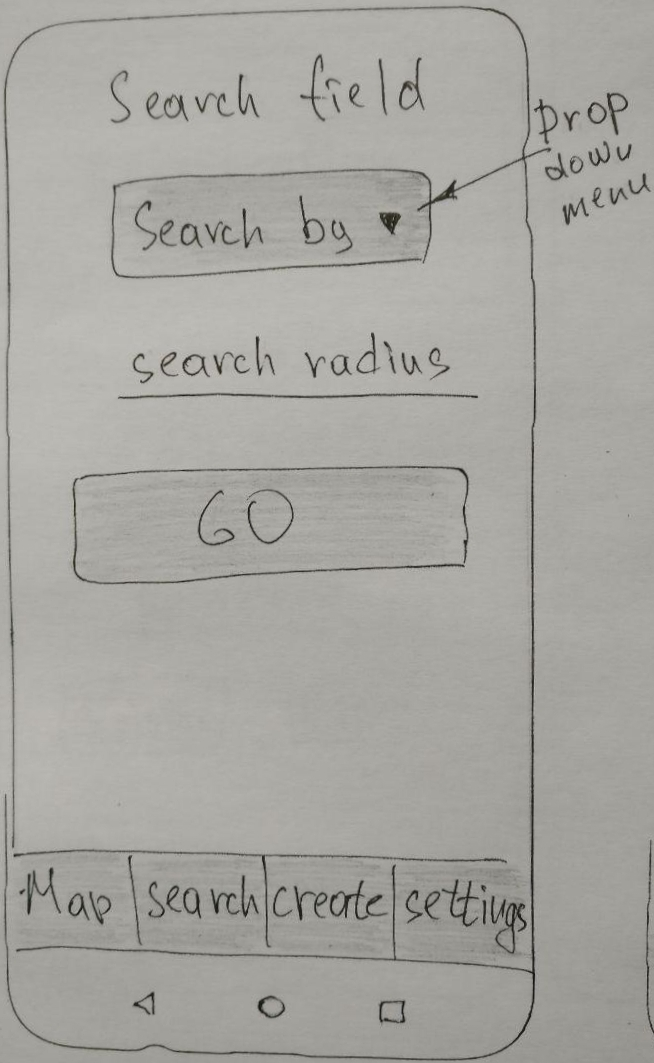
\includegraphics[width=0.30\linewidth]{rys02/search_makiet.jpg}}} &
	b) & \vtop{\vskip-2ex\hbox{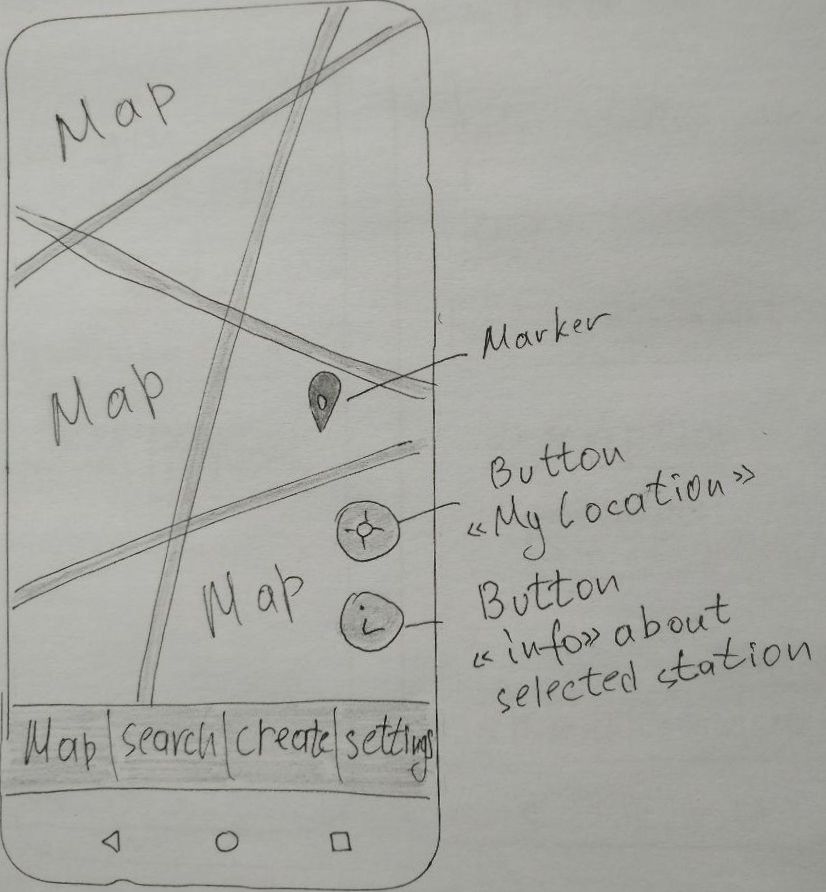
\includegraphics[width=0.45\linewidth]{rys02/main_makiet.jpg}}} 
		\end{tabular}
        \caption{Makiety interfejsów aplikacji mobilnej: a) strona wyszukiwania stacji ładowania, b) strona główna.}
    \label{fig:search_makiet}
\end{figure}

Na rysunku~\ref{fig:search_makiet}b przedstawiono makietę pozwalającą dokonać wyboru stacji ładowania. Stacje poznaczone znacznikami na mapie. Dla otrzymania informacji o wybranej stacji (wybierany jest markier na mapie) oraz wyświetlania pozycji użytkownika wykorzystują się okrągłe przyciski z lewej strony ekranu.

Podczas tworzenia stacji ładowania (rys. \ref{fig:create_makiet}) dla wygody użytkowania można wybrać miejsce na mapie poprzez odpowiedni przycisk.
\begin{figure}[ht]
    \centering
        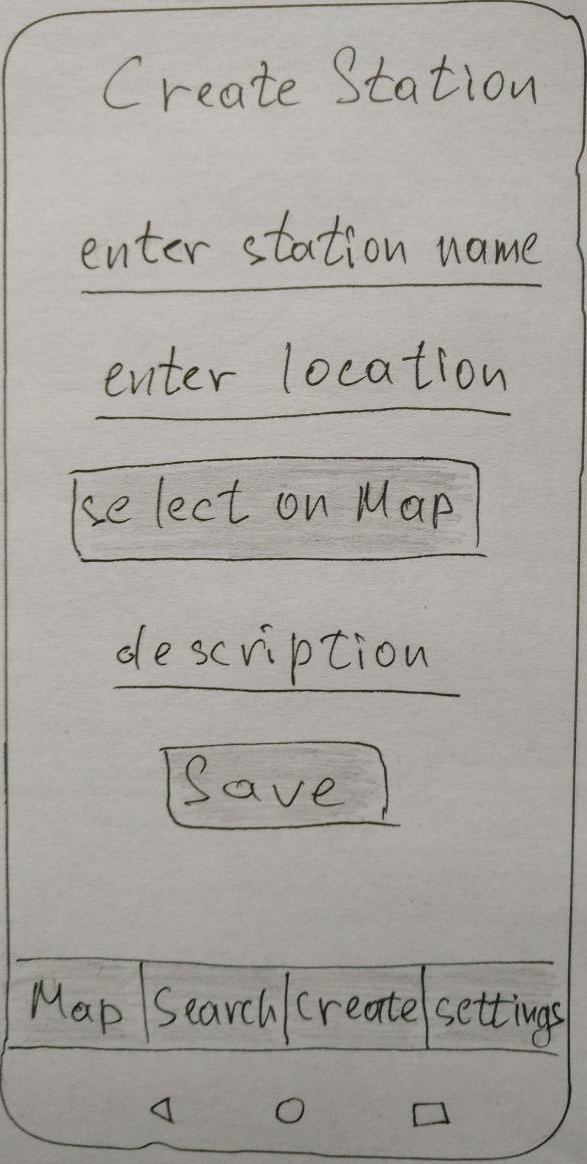
\includegraphics[width=0.3\linewidth]{rys02/create_makiet.jpg}
        \caption{makiet strony tworzenia stacji ładowania}
    \label{fig:create_makiet}
\end{figure}
\newpage
Na stronie informacji o stacji (rys.\ref{fig:station_makiet}) oprócz nazwy stacji, opisu oraz oceny, wyliczonej na podstawie komentarzy oceny, znajdują się komentarzy uzytkowników w porządku: najpierw najnowsze.
% TO DO: proszę ułożyć dwie makiety obok siebie, jak w przykładzie powyżej
\begin{figure}[ht]
    \centering
        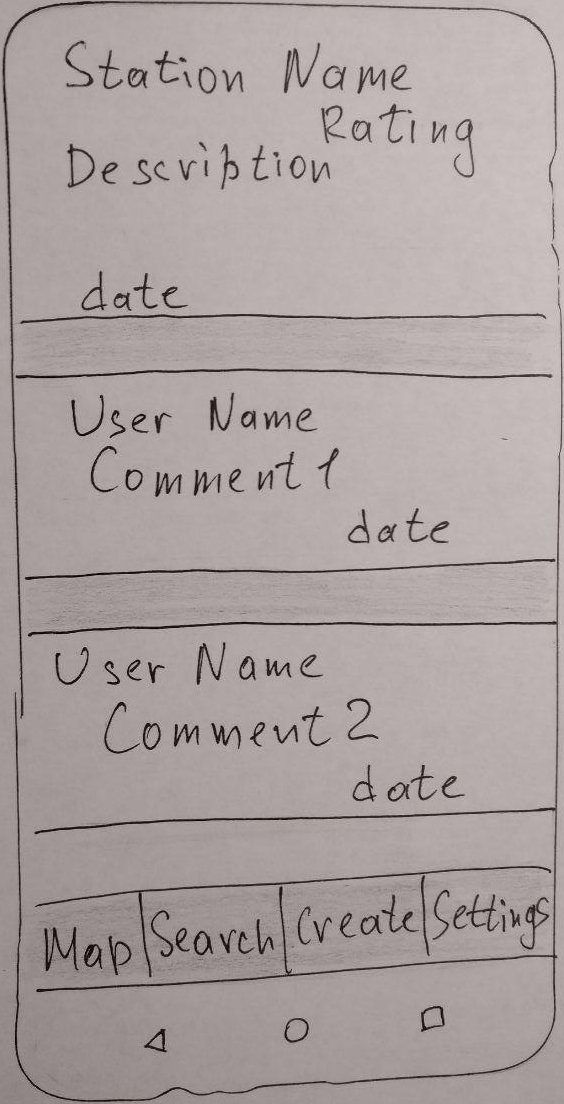
\includegraphics[width=0.3\linewidth]{rys02/station_makiet.jpg}
        \caption{makiet strony informacji o stacji ładowania}
    \label{fig:station_makiet}
\end{figure}
\newline
Dla rejestracji i logowania wykorzystują się dwa różne ekrany (rys.\ref{fig:login_makiet} oraz \ref{fig:register_makiet})
\begin{figure}[ht]
    \centering
        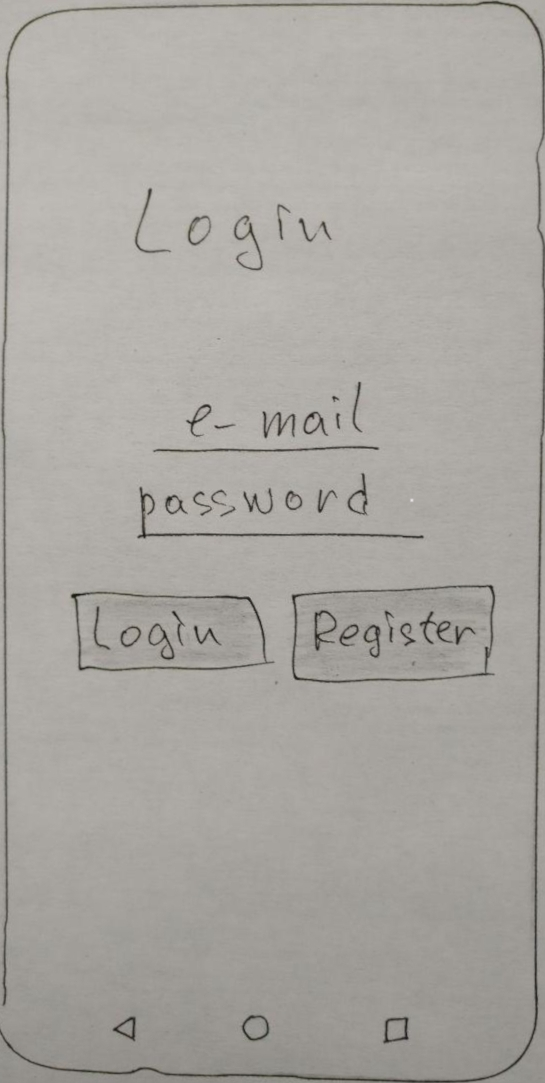
\includegraphics[width=0.3\linewidth]{rys02/login_makiet.jpg}
        \caption{makiet strony logowania}
    \label{fig:login_makiet}
\end{figure}
\begin{figure}[ht]
    \centering
        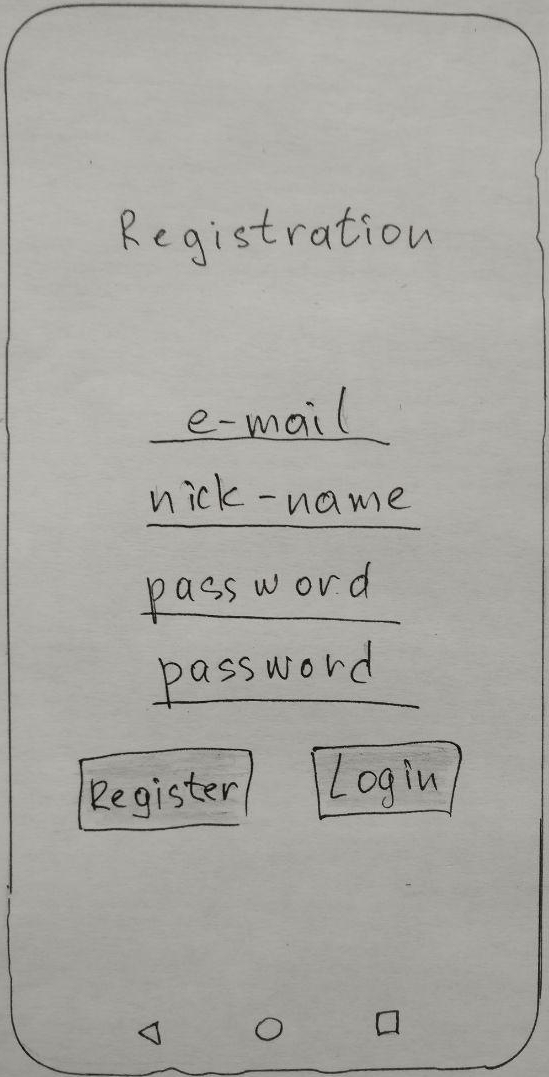
\includegraphics[width=0.3\linewidth]{rys02/register_makiet.jpg}
        \caption{makiet strony rejestracji}
    \label{fig:register_makiet}
\end{figure}
\newpage



% \paragraph{Część serwerowa:}
% \begin{itemize}
%     \item Visual Studio Code
%     \item Go
%     \item MongoDB
%     \item Redis
%     \item Docker ?
%     \item Docker-compose ?
%     \item Go Modules
%     \item gorilla/mux
%     \item sirupsen/logrus
%     \item mongo-driver
%     \item go-redis/redis
%     \item go-ozzo/ozzo-validation
%     \item yaml.v2
%     \item google/uuid
% \end{itemize}

% \paragraph{Aplikacja mobilna:}
% \begin{itemize}
%     \item Android Studio
%     \item Java   
%     \item ? gradle ?
%     \item RxJava
%     \item OkHttp 3
%     \item Retrofit 2
%     \item Maps SDK for Android
%     \item Google Play services APIs
%     \item gson
% \end{itemize}

% \paragraph{Testowanie: ??}
% \begin{itemize}
%     \item Postman
%     \item MongoDB Compass
%     \item stretchr/testify ??
% \end{itemize}


% \paragraph{Paragraf}
% Tekst\newline
% Tekst
